\documentclass[11pt]{jarticle}

%パッケージ
\usepackage{amssymb,amsmath}
\usepackage{listings}
\usepackage[dvipdfmx]{graphicx}
%レイアウト
\setlength{\oddsidemargin}{0mm}
\setlength{\textwidth}{160mm}
\setlength{\topmargin}{-9mm}
\setlength{\headheight}{0mm}
\setlength{\textheight}{241mm}
\lstset{
  language=Lisp,
  frame=tblr,
  commentstyle=\ttfamily,
  morekeywords={
    if, define
  }
}
%%%%%%%%%%%%%%%%%%%%%%%%%%%%%%%%%%%%%%%%%%%%%%%%%%
\begin{document}

%%%%%%%%%%%%%%%%%%%%%%%%%%%%%%%%%%%%%%%%%%%%%%%%%%
%%% Header
\begin{flushleft}
  中間発表\hspace{\fill}
  恩田晴登 (2022年7月26日)
\end{flushleft}
\begin{center}
{\Large\bf Docker,Kubernetes}
\end{center}

%%%%%%%%%%%%%%%%%%%%%%%%%%%%%%%%%%%%%%%%%%%%%%%%%%
\section{仮想化マシンとコンテナ}

仮想環境は、「安全で効率的なアプリの開発や運用」を行うために使用する。チームでアプリを開発する際、様々なケースでアプリが使われるが、
1つのサーバやPC上に必要とされる仮想環境を構築しておくことで、様々な用途で自由にアプリを使用できるようになる。

コンテナとは、サーバ内を整理してアプリケーションやWebの開発・管理を効率的に行えるようにする仮想化技術である。
従来の仮想化マシンは、1つの仮想環境の中に必要なものをOSから全て作っていたが、コンテナ環境ではOS周辺の環境は共通で使用し、
アプリが使用するCPU、メモリ、ファイルなどは別々にまとまったコンテナとして管理する。これにより、OS関連でリソース削減ができ、
軽量のサーバでも仮想環境が作成できるという大きなメリットに繋がる。

\begin{figure}[ht]
  \centering
  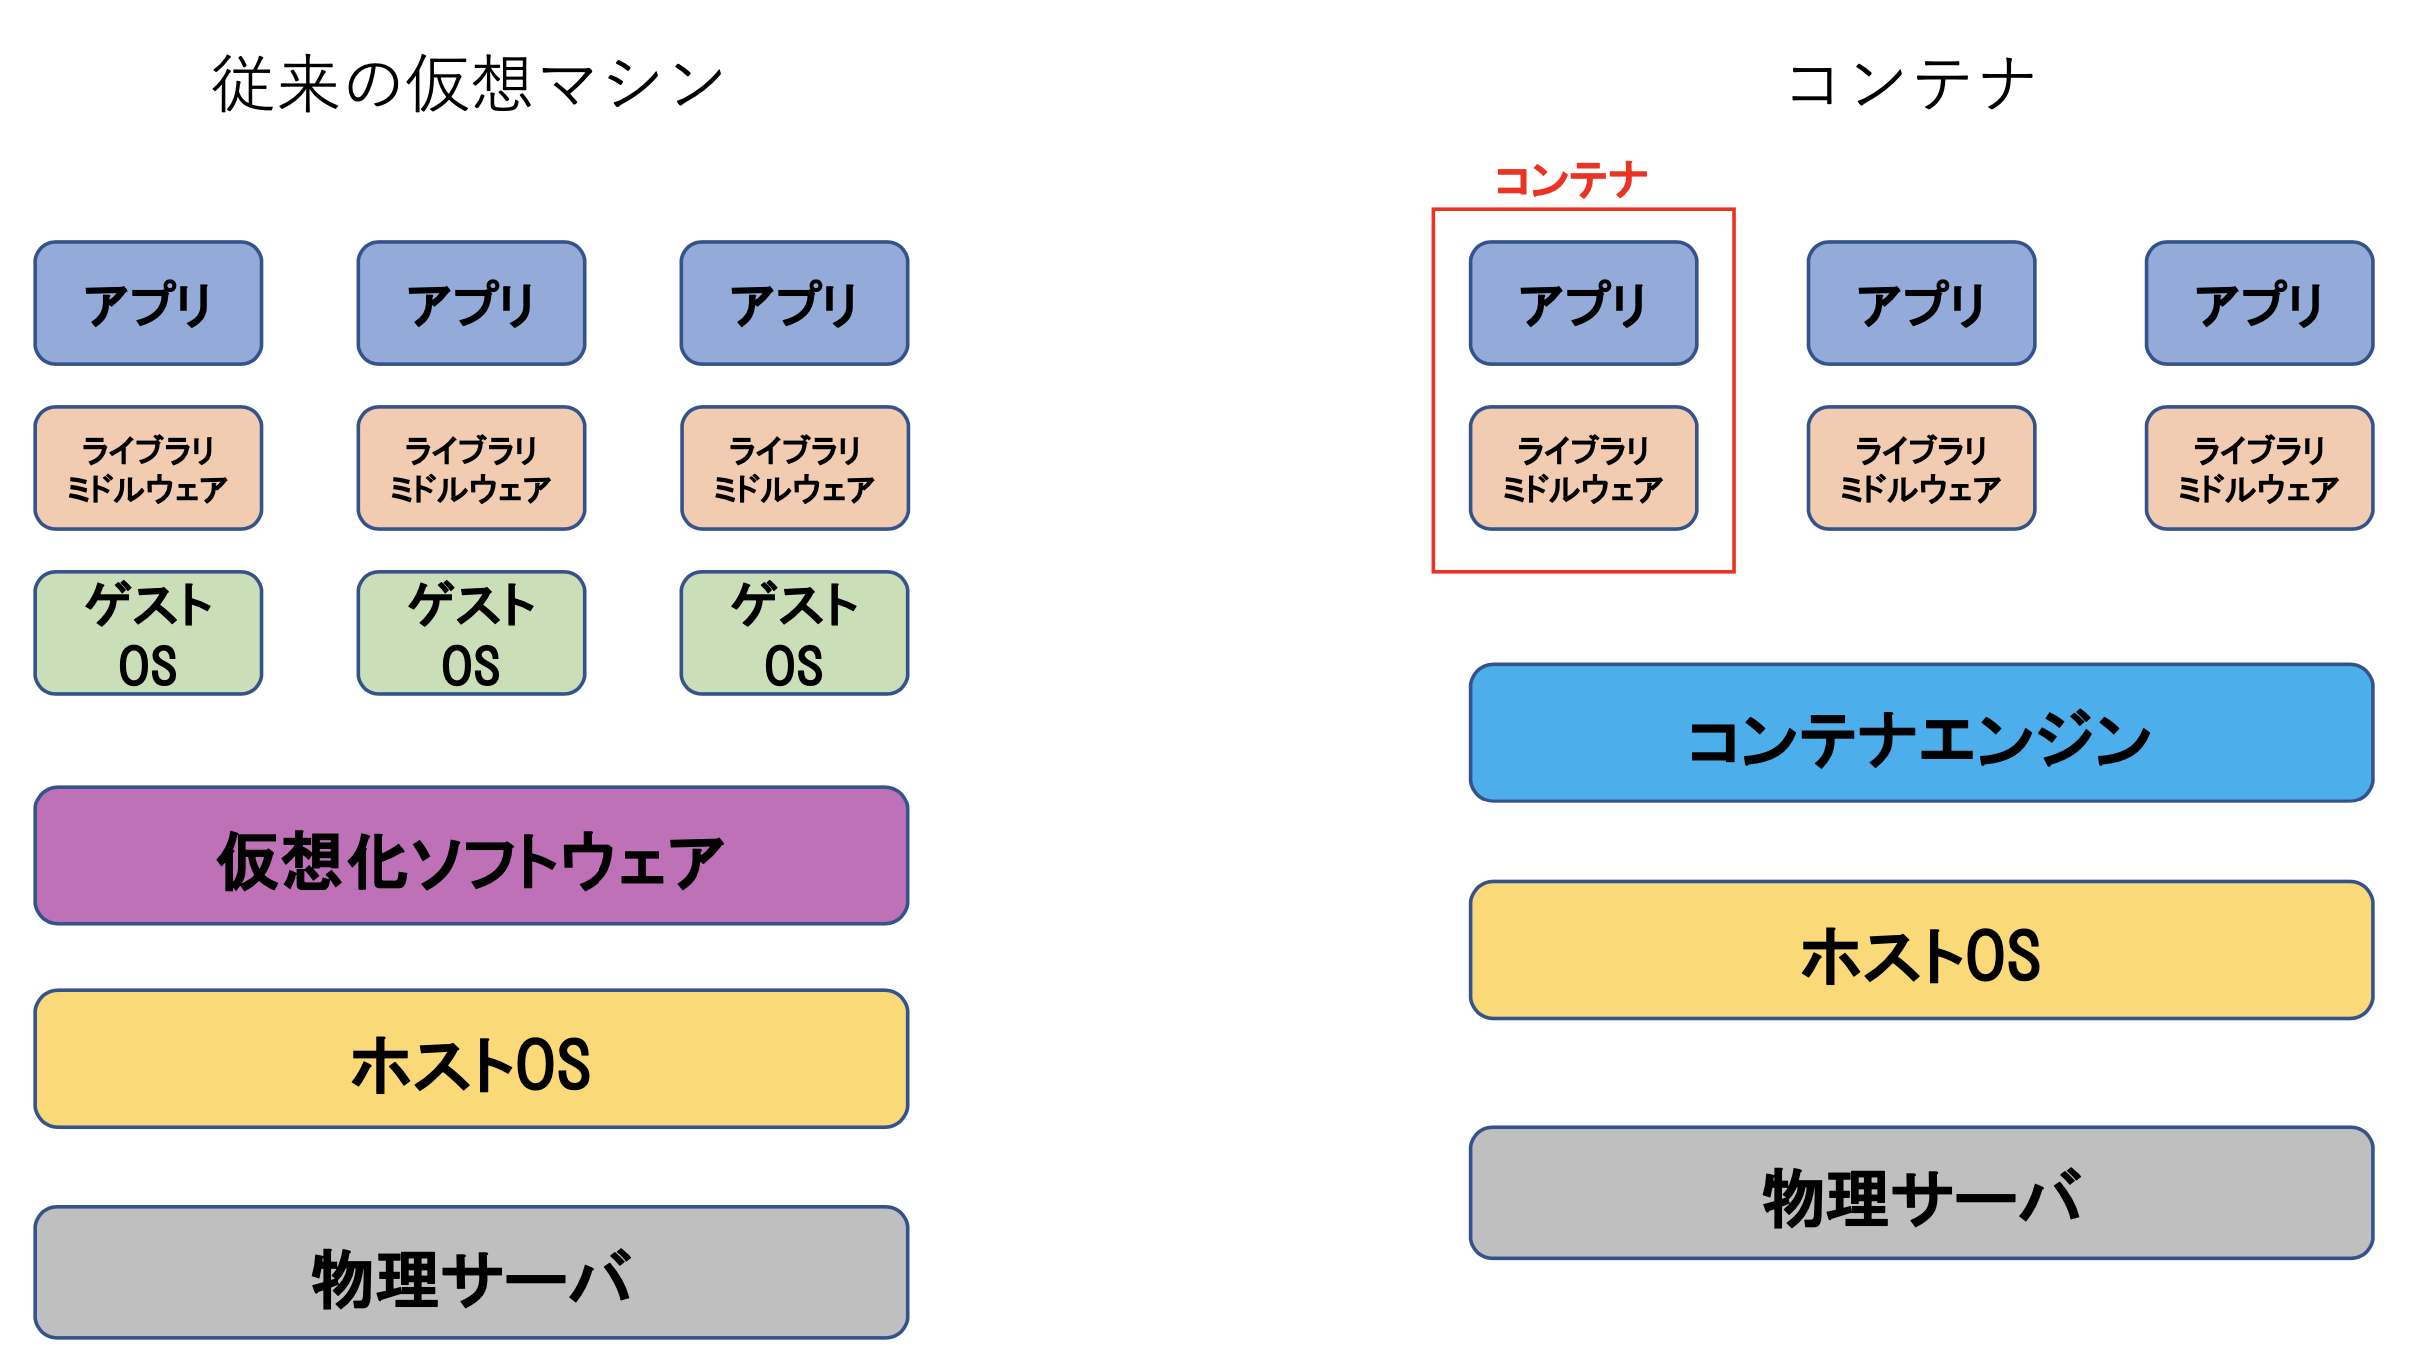
\includegraphics[keepaspectratio, scale=0.25]{container.png}
\end{figure}

\subsection{Docker}

DockerはLinuxOSの元でコンテナを使える仕組みの一つで、主にサーバで使われる。
Dockerはミドルウェアのインストールや各種環境設定をコード化(Dockerfile)して管理するため、開発環境によるバージョンのずれ防止や開発環境準備の短縮化をすることが可能になる。
Dockerは基本Linuxで動くが、WindowsやMacでもデスクトップ版が存在し、仮想のLinux環境を作ってDocker Engineが使える。

\subsection{Kubernetes}

KubernetesはDockerなどのコンテナ仮想化ソフトウェアを管理、および自動化するためのオープンソースのプラットフォームである。
コンテナには、アプリケーションを実行する機能はあるが、コンテナを管理したり、他のサーバと連携させたりする機能はなく、それを解決するのがKubernetesである。
Dockerは1台の物理マシンの上にコンテナを作り実行していくのに対し、Kubernetesは複数の物理マシンを扱うことが前提である。Kubernetes内で作ったマニフェストファイルに従い、
複数の物理マシンにおけるコンテナの作成や管理の煩雑さを自動的に処理する。
%%%%%%%%%%%%%%%%%%%%%%%%%%%%%%%%%%%%%%%%%%%%%%%%%%
\section{現在の進捗}\mbox{}\\
・DockerとKubernetesの基本を学んだ。(DockerDesktopでのコンテナの操作、Kubernetesのマニフェストファイルの記述など)
\\
・Kubernetesのチュートリアルとして、Redisを使用したPHPゲストブックアプリケーションのデプロイを実行した。\cite{redis}
%%%%%%%%%%%%%%%%%%%%%%%%%%%%%%%%%%%%%%%%%%%%%%%%%%
\section{今後の課題}\mbox{}\\
・研究分野への活用を考える(過去の論文や制作物などから知見を得る)。
\\
・DockerとKubernetesを使ったアプリケーションなどや、使用例から更なる学習をする。
\\
・Kubernetesが使用されているマイクロサービスについて学習する。

%%%%%%%%%%%%%%%%%%%%%%%%%%%%%%%%%%%%%%%%%%%%%%%%%%
\begin{thebibliography}{99}
  \bibitem{redis} Kubernetes. https://kubernetes.io/ja/docs/tutorials/
\end{thebibliography}
\end{document}

